\chapter{Технология кросс-архитектурной миграции}

\section{Верхнеуровневая архитектура}

\begin{figure}[h]
\center{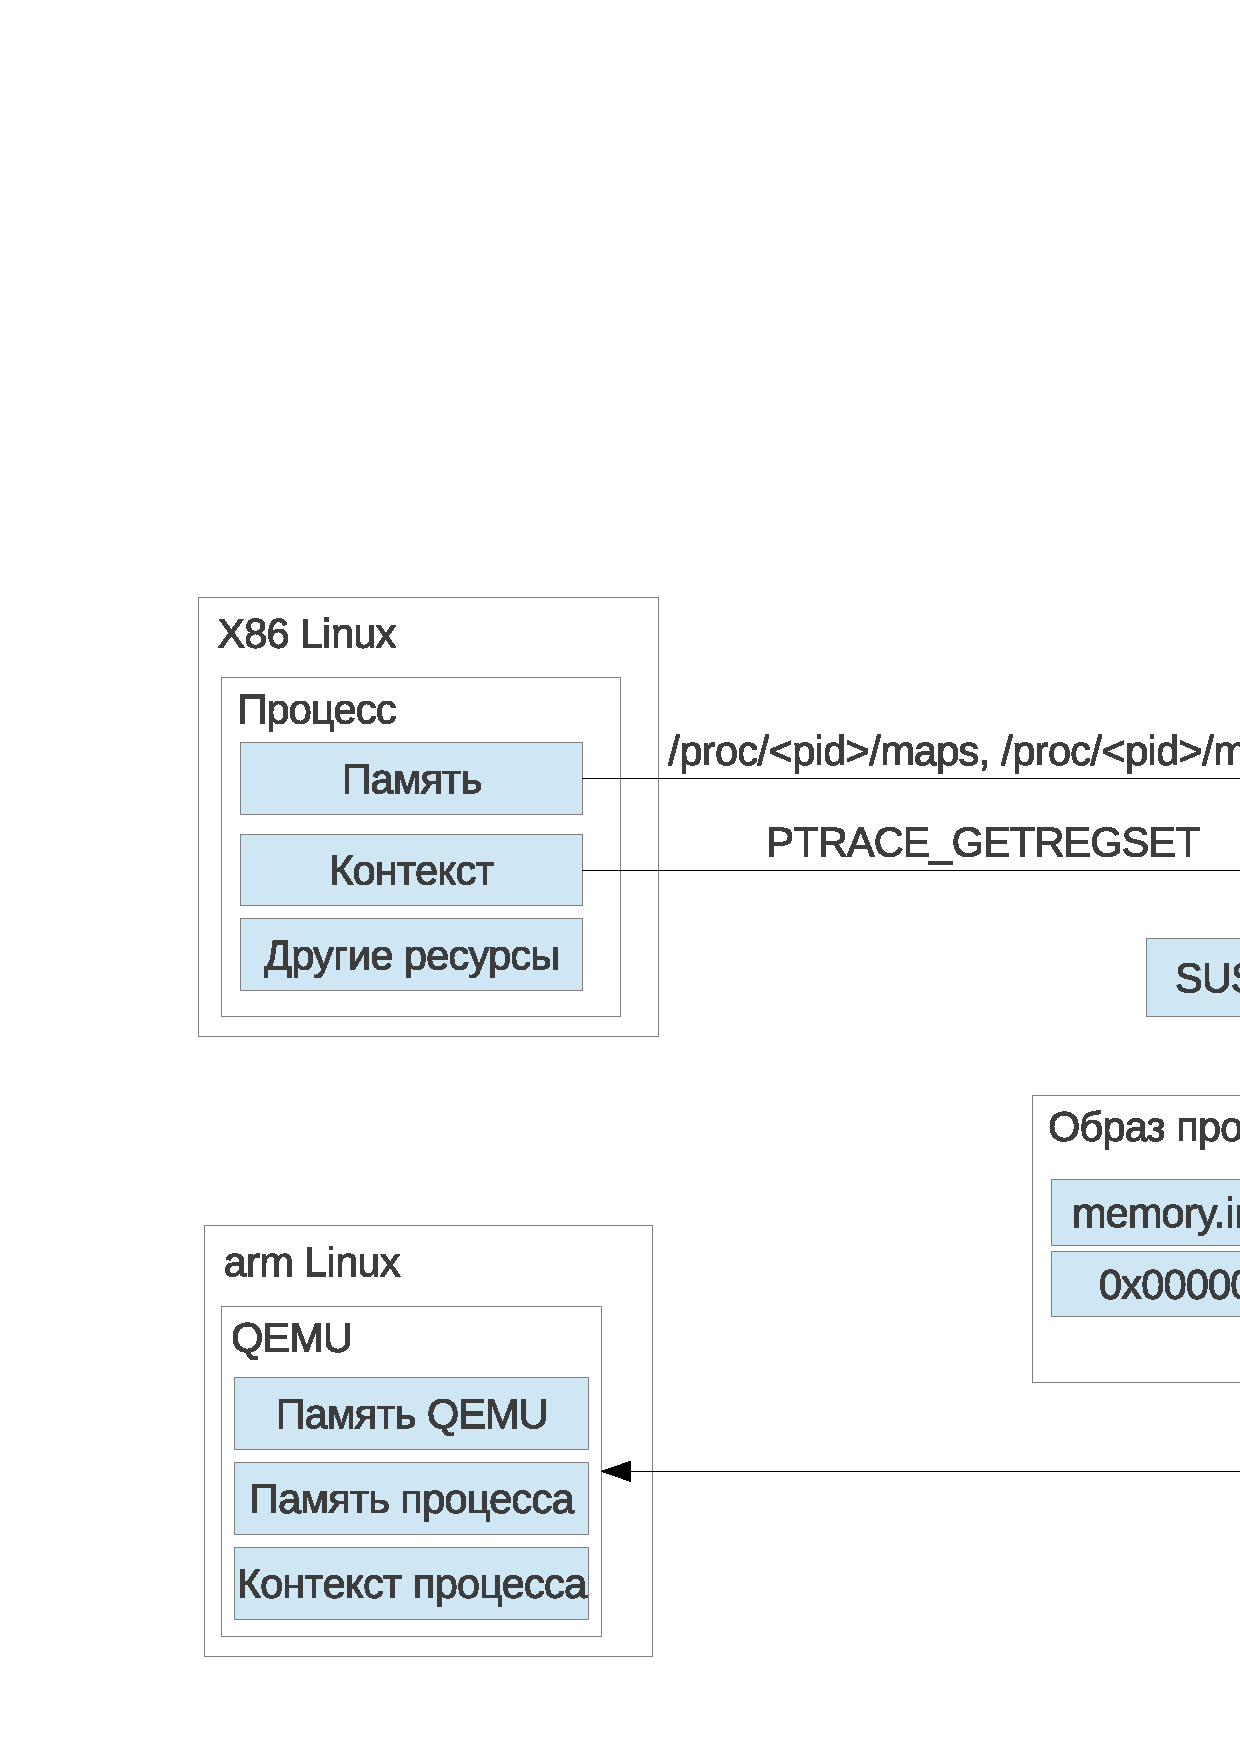
\includegraphics[width=1\linewidth]{common_arch}}
\caption{Верхнеуровневая архитектура}
\label{pic:common_arch}
\end{figure}

На рис.~\ref{pic:common_arch} изображены основные компоненты системы.

\paragraph{SUSPEND Tool.}

Задача приложения собрать информацию о процессе и сохранить ее в виде набора файлов. В данной работе рассматриваются только два ресурса процесса - состояние регистров и состояние памяти.

Для доступа к информации о процессе используются интерфейсы ОС Linux - системный вызов \textit{ptrace} и файловая система \textit{proc} (в частности два файла \textit{maps} и \textit{mem}).

\paragraph{QEMU.}

В качестве динамического транслятора выступает QEMU. В данной работе внесены изменения в QEMU User Mode, чтобы была возможность не только создавать процесс заново, но восстанавливать процесс по образу.

Для восстановления процесса необходимо зарезервировать область под память гостевого процесса и заполнить ее содержимым памяти из образа процесса, а также заполнить значениями из образа поля виртуального окружения QEMU.

\paragraph{Формат хранения данных.}

Для описания формата хранения данных используется Protobuf~\footnote{https://code.google.com/p/protobuf/}, который позволяет по описание формата сгенерировать сгенерировать код разбора и сохранения описанной структуры.

Описание контекста сохраняется в файле \textit{registers.img}, описание регионов памяти сохраняется в файле \textit{memory.img}, кроме того для каждого региона памяти выделен отдельный файл, хранящий непосредственно содержимое региона памяти.

\section{Останов процесса}

\subsection{Архитектура}

\begin{figure}[h]
\center{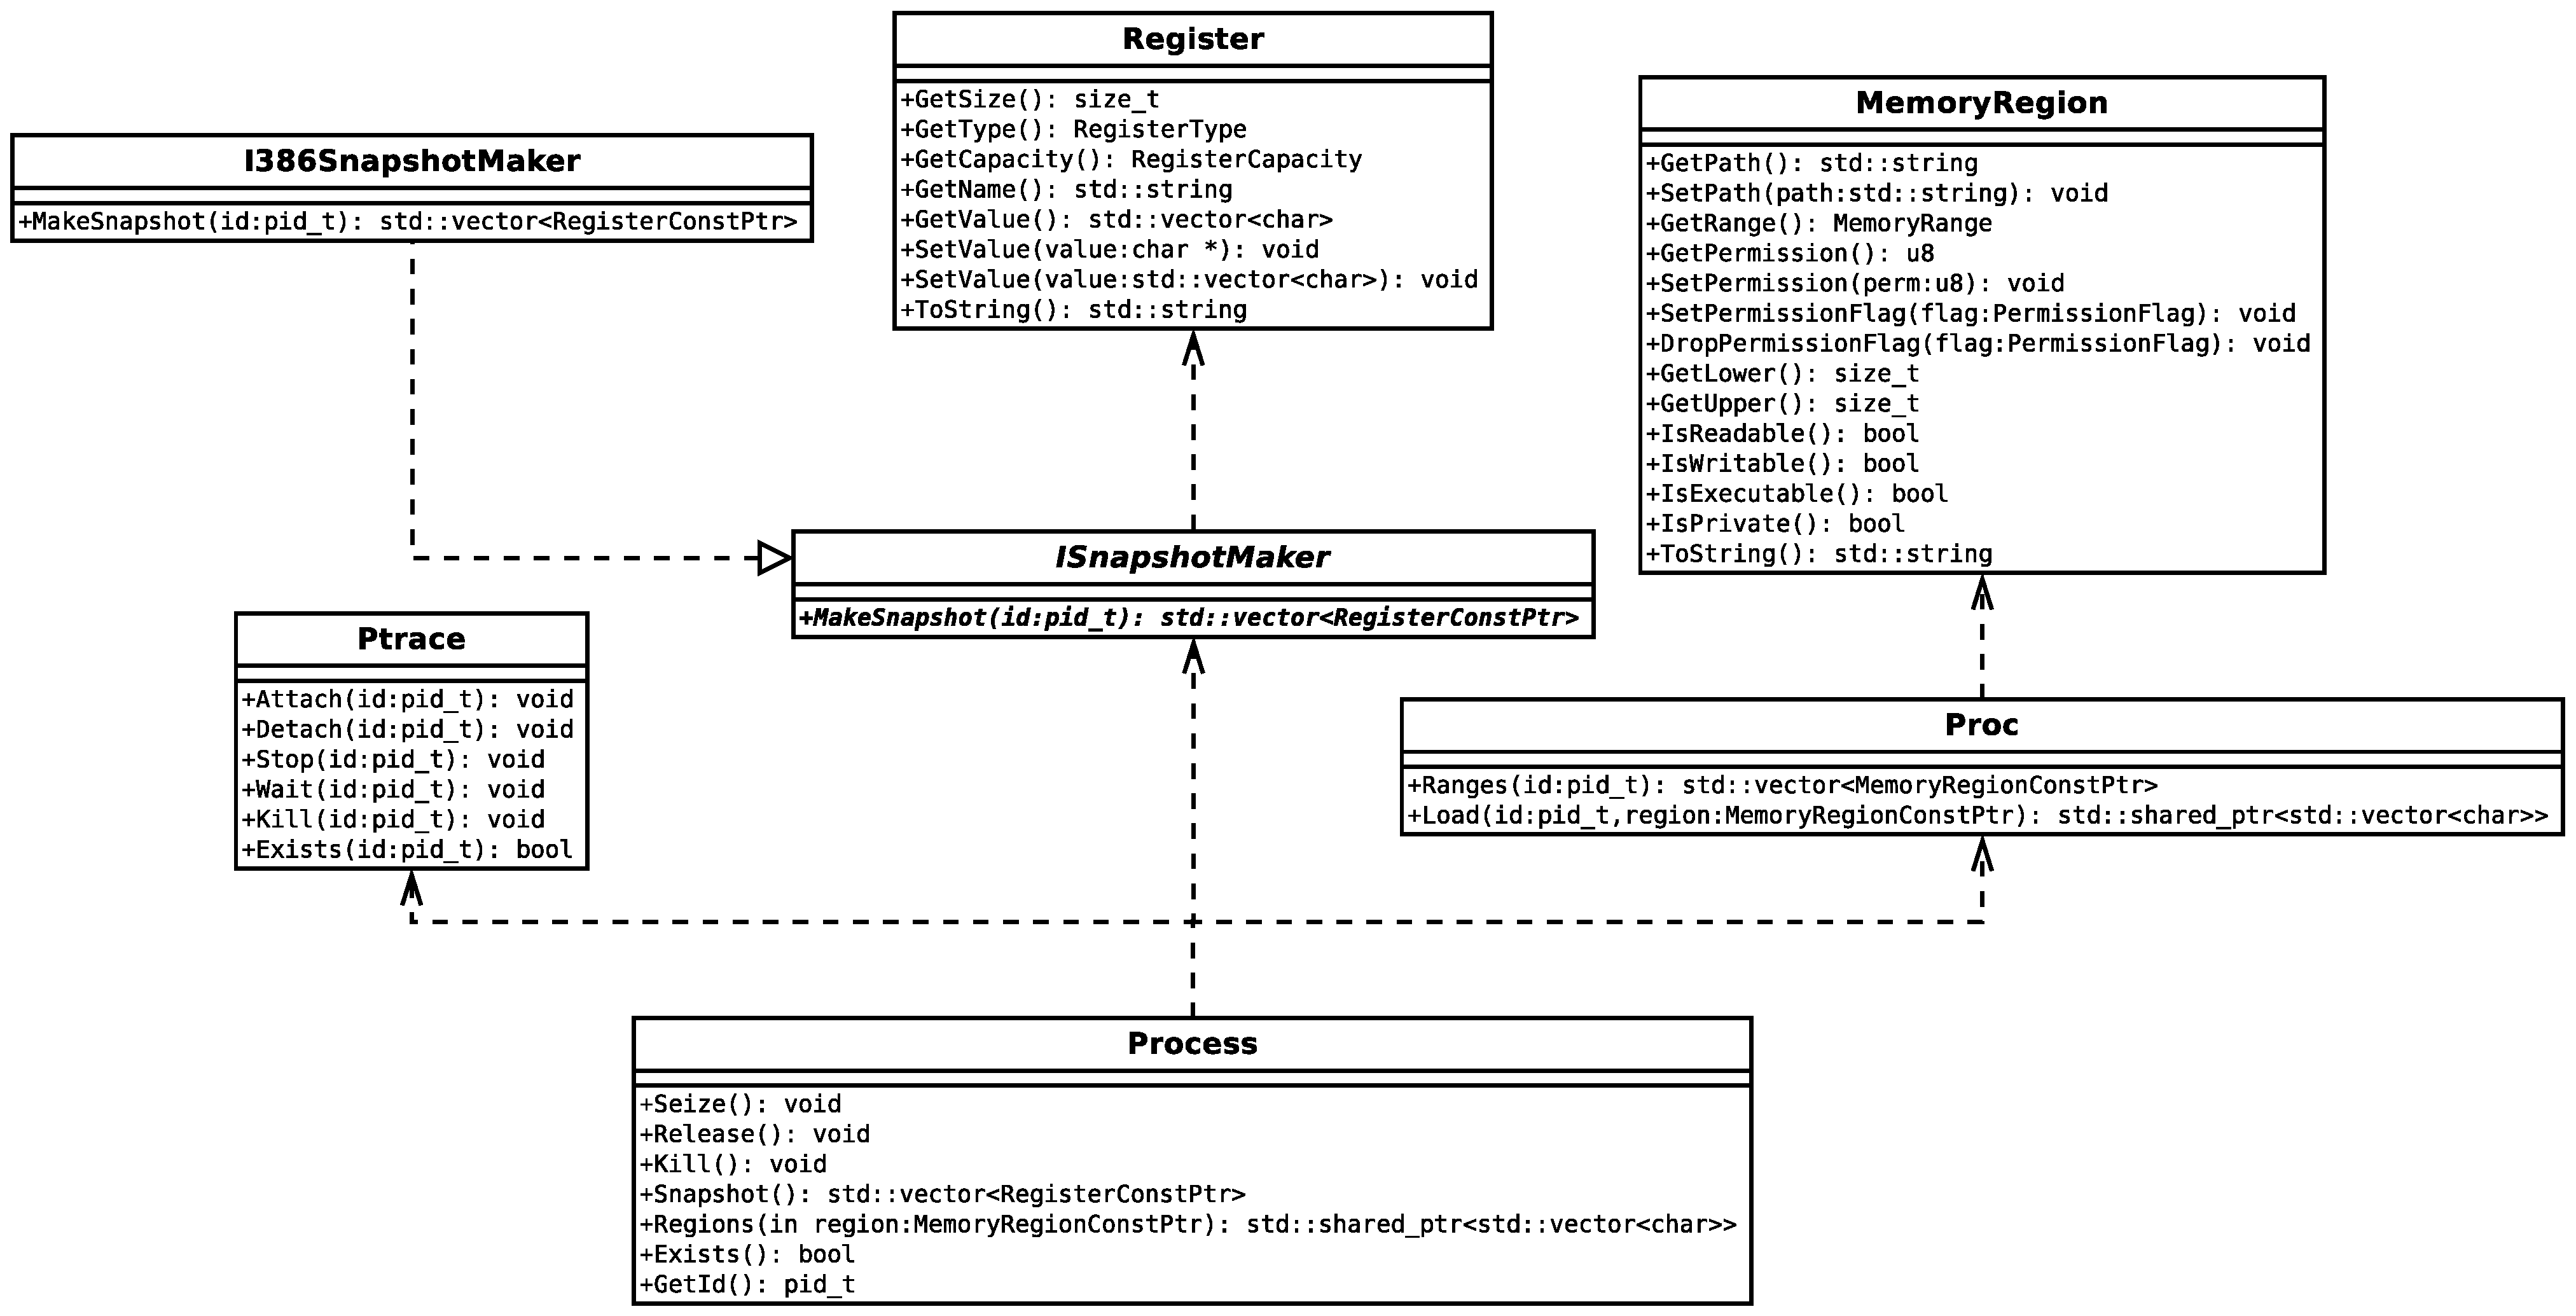
\includegraphics[width=1\linewidth]{suspend_arch}}
\caption{Архитектура утилиты создания образа процесса}
\label{pic:suspend_arch}
\end{figure}

На рис.~\ref{pic:suspend_arch} представлены главные компоненты приложения для создания образа процесса.

\paragraph{Process.}

Абстракция процесса - класс предоставляющий единый архитектурно-независимый интерфейс для захвата и останова процесса, а также для получения его ресурсов. Класс \textit{Process} зависит от трех компонентов: \textit{ptrace}, \textit{proc} и \textit{ISnapshotMaker}.

\paragraph{Ptrace.}

Обертка над системным вызовом \textit{ptrace}, она предоставляет интерфейс к независимым от архитектуры командам \textit{ptrace}.

\paragraph{Proc.}

Интерфейс к файловой системе \textit{proc}, для получения информации о памяти процесса.

\paragraph{ISnapshotMaker.}

Контекст исполнения процесса получается с помощью системного вызова \textit{ptrace}, однако набор регистров отличен для различных платформ, поэтому получение состояния регистров выделено в отдельный интерфейс. Задача \textit{ISnapshotMaker} сделать снимок регистров и привести его к архитектурно независимому виду.

Чтобы поддержать другую аппаратную платформу в приложении (например, arm), потребуется реализовать интерфейс \textit{ISnapshotMaker} и зарегистрировать его с помощью макроса \textit{DECLARE\_IMPLEMENTATION}.

\subsection{Системный вызов ptrace}

\begin{lstlisting}[caption=Вызов ptrace, label=code:ptrace]
    #include <sys/ptrace.h>
    long ptrace(enum __ptrace_request request, pid_t pid, ...);
\end{lstlisting}

Системный вызов \textit{ptrace} (см. листинг~\ref{code:ptrace}) предоставляет широкие возможности по отслеживанию состояния процесса, а также позволяет изменять состояние процесса прямо во время работы, эту возможность, например, активно использует дебагер \textit{gdb}.

В листинге~\ref{code:ptrace}:

\begin{itemize}

    \item \textit{request} - номер команды для выполнения
    \item \textit{pid} - id целевого процесса

\end{itemize}

В данной работе \textit{ptrace} используется для захвата и останова процесса, а также для получения снимка регистров процесса.

\paragraph{Захват процесса.}

Для захвата процесса существуют следующие команды \textit{ptrace}: \textit{PTRACE\_TRACEME}, \textit{PTRACE\_ATTACH}.

\begin{itemize}

    \item \textit{PTRACE\_TRACEME} - после этой команды родительский процесс может наблюдать за процессом из которого был произведен вызов. Типичное использование - запуск приложения под отладчиком, после того как отладчик сделал \textit{fork}, но перед \textit{exec}, отладчик в порожденном процессе исполняет команду \textit{PTRACE\_TRACEME}, таким образом захватывая порожденный процесс.

    \item \textit{PTRACE\_ATTACH} - позволяет произвольному процессу подключаться к любому другому процессу, идентификатор которого передается в параметре \textit{pid}. Для исполнения этой команды процесс должен быть запущен с правами суперпользователя.

\end{itemize}

\paragraph{Останов процесса.}

Для останова процесса используется команда \textit{PTRACE\_INTERRUPT}. Надо отметить, что это не единственная команда позволяющая остановить процесс, но в отличие от команды \textit{PTRACE\_STOP} или команд остановки по условию она не создает дополнительных побочных эффектов (например, посылки сигналов или каких-либо других эффектов влияющих на работу целевого процесса).

\paragraph{Получение списка регистров.}

Для получения списка регистров используется команда \textit{PTRACE\_GETREGSET}. В дополнительном аргументе передается константа описывающие набор регистров (например, константа \textit{NT\_PRSTATUS} используется для получения "основного" набора регистров, а константа \textit{NT\_PRFPREG} для получения регистров FPU).

\begin{lstlisting}[caption=Основной набор регистров, label=code:general]
    struct user_regs_struct32 {
        __u32 ebx, ecx, edx, esi, edi, ebp, eax;
        unsigned short ds, __ds, es, __es;
        unsigned short fs, __fs, gs, __gs;
        __u32 orig_eax, eip;
        unsigned short cs, __cs;
        __u32 eflags, esp;
        unsigned short ss, __ss;
    };
\end{lstlisting}

Основной набор регистров, который используется в работе описывается структурой из листинга~\ref{code:general}. Для представления регистров в программе используется класс \textit{Register} (см. рис.~\ref{pic:arch}). Преобразованием структуры из листинга~\ref{code:general} в вектор объектов класса \textit{Register} занимается класс \textit{I386SnapshotMaker} реализующий интерфейс \textit{ISnapshotMaker}.

\begin{lstlisting}[caption=Формат сохранения регистров, label=code:regs_proto]
    package protobuf;

    message Register {
        required string name = 1;
        enum Type {
            INTEGER = 0;
            FLOATING_POINT = 1;
        }
        required Type type = 2;
        enum Capacity {
            BIT8 = 8;
            BIT16 = 16;
            BIT32 = 32;
            BIT64 = 64;
            BIT128 = 128;
        }
        required Capacity capacity = 3;
        required bytes value = 4;
    }

    message RegistersSnapshot {
        repeated Register register = 1;
    }
\end{lstlisting}

Формат сохранения состояния регистров определяется файлом описания protobuf из листинга~\ref{code:regs_proto}. Код сохранения и чтения генерируется с помощью компилятора protoc во время сборки проекта.


\subsection{Файловая система proc}

\begin{lstlisting}[caption=Формат файла maps, label=code:maps]
08048000-08057000 r-xp 00000000 08:03 5899468    /usr/bin/update-notifier

...

08863000-08bae000 rw-p 00000000 00:00 0          [heap]
41000000-41020000 r-xp 00000000 08:03 5636122    /lib/i386-linux-gnu/ld-2.15.so
41020000-41021000 r--p 0001f000 08:03 5636122    /lib/i386-linux-gnu/ld-2.15.so

...

411ca000-411cb000 rw-p 001a5000 08:03 5636768    /lib/i386-linux-gnu/libc-2.15.so
411cb000-411ce000 rw-p 00000000 00:00 0 
4342d000-43527000 r-xp 00000000 08:03 5636775    /lib/i386-linux-gnu/libglib-2.0.so.0.3400.1
43527000-43528000 r--p 000f9000 08:03 5636775    /lib/i386-linux-gnu/libglib-2.0.so.0.3400.1

...

b77e6000-b77e8000 rw-p 00000000 00:00 0 
b77e8000-b77e9000 r-xp 00000000 00:00 0          [vdso]
bfc44000-bfc65000 rw-p 00000000 00:00 0          [stack]
\end{lstlisting}

\textit{proc} - виртуальная файловая система предоставляющая информацию о процессах. Каждому процессу в файловой системе \textit{proc} соответствует директория \textit{/proc/<pid>}, где \textit{<pid>} - идентификатор процесса. В работе я использую файловую систему \textit{proc} для доступа к памяти процесса.

Внутри ядра Linux информация о каждом регионе памяти процесса хранится в структуре \textit{vm\_area\_struct}, все регионы объединены в список упорядоченный по начальному адресу региона, указатель на голову списка хранится в структуре \textit{mm\_struct} в поле \textit{mmap} (см. листинг~\ref{code:mm_struct}). В пространстве пользователя доступ к этой информации может быть осуществлен через файл \textit{maps}, который имеет формат представленный в листинге~\ref{code:maps}: 

\begin{enumerate}

    \item столбец содержит адреса занимаемые регионом памяти [начальный; конечный).

    \item столбец описывает права региона памяти:

        \begin{itemize}

            \item r (read) - регион доступен для чтения
            \item w (write) - регион доступен для записи
            \item x (execute) - регион может содержать исполянемый код
            \item p (private) - регион приватный, т. е. не разделяется с другими процессами

        \end{itemize}

    \item столбец описывает смещение в файле, если регион - файл отображенный в память, и содержит 0 в противном случае.

    \item столбец содержит минорный и мажорный номер устройства, на котором находится файл, если регион - отображенный в память файл.

    \item столбец содержит \textit{inode} соответствующий отображенному файлу и 0 в противном случае

    \item столбец содержит путь к отображенному файлу или назначение региона памяти (например, \textit{[heap]} или \textit{[stack]}).

\end{enumerate}

По каждой строке файла \textit{maps} создается описатель региона памяти \textit{MemoryRegion} (см. рис.~\ref{pic:common_arch}). Описатели всех регионов памяти сохраняются в файл \textit{memory.img}. Формат файла описывается файлом protbuf из листинга~\ref{code:maps_proto}.

\begin{lstlisting}[caption=Формат сохранения описателей регионов памяти, label=code:maps_proto]
    package protobuf;

    message MemoryRegion {
        required uint64 lower = 1;
        required uint64 upper = 2;
        required string path = 3;

        required bool readable = 4;
        required bool writable = 5;
        required bool executable = 6;
        required bool shared = 7;
    }

    message MemoryRegions {
        repeated MemoryRegion region = 1;
    }
\end{lstlisting}

Непосредственно память процесса доступна через файл \textit{mem}. Байту со смещением \textit{x} в адресном пространстве процесса соответствует байт со смещением \textit{x} в файле \textit{mem}. Попытка доступа к файлу со смещением не попадающим не в один из регионов памяти приводит к ошибке. Так как целевой процесс может занимать много памяти, содержимое регионов памяти загружается по требованию, после чего сразу же сохраняется в соответствующий файл на диске, а память освобождается.

\newpage
\subsection{Организация проекта и система сборки}

Конфигурация проекта и сборка осуществляется посредством системы CMake~\footnote{http://www.cmake.org/}. Организация директорий представлена в листинге~\ref{code:dirs}

\begin{lstlisting}[caption=Организация каталогов, label=code:dirs]
    +- inc/ +- process/ +- {memory.h, process.h, registers.h, serialize.h}
    |       |           |
    |       |           +- proc/ +- proc.h
    |       |           |
    |       |           +- ptrace/ +- ptrace.h, snapshot.h
    |       |                      |
    |       |                      +- i386/ +- snapshot.h
    |       |
    |       +- utils/ +- {casts.h, exceptions.h, range.h, string_utils.h, types.h}
    |       |
    |       +- i386/ +- types.h
    |
    +- src/ +- core/ +- main.cpp
            |
            +- lib/ +- serialize.cpp
            |       |
            |       +- process/ +- proc/ +- proc.cpp
            |                   |
            |                   +- ptrace/ +- ptrace.cpp
            |                              |
            |                              +- i386/ +- snapshot.cpp
            |
            +- protobuf/ +- {memory.proto, snapshot.proto}
            |
            +- test/ +- {casts.cpp,  protobuf.cpp, registers.cpp, string_utils.cpp}
\end{lstlisting}

Проект имеет следующие зависимости

\begin{itemize}

    \item Boost unit\_test\_framework
    \item Boost program\_options
    \item Boost regex
    \item Protobuf

\end{itemize}

\begin{lstlisting}[caption=Генерация исходных кодов по файлам описания protobuf, label=code:custom_command]
set(PROTO_SRC ${MANTICORE_LIBRARY_DIR}/snapshot.pb.cc ${MANTICORE_LIBRARY_DIR}/memory.pb.cc)
set(PROTO_HDR ${MANTICORE_LIBRARY_DIR}/snapshot.pb.h ${MANTICORE_LIBRARY_DIR}/memory.pb.h)
list(APPEND PROTO_FILES_ALL ${PROTO_HDR})
list(APPEND PROTO_FILES_ALL ${PROTO_SRC})
add_custom_target(protogen)
add_custom_command(
	TARGET protogen
	COMMAND protoc
	ARGS -I=${MANTICORE_PROTOBUF_DIR} --cpp_out=${MANTICORE_LIBRARY_DIR} ${MANTICORE_PROTOBUF_DIR}/snapshot.proto
)
add_custom_command(
	TARGET protogen
	COMMAND protoc
	ARGS -I=${MANTICORE_PROTOBUF_DIR} --cpp_out=${MANTICORE_LIBRARY_DIR} ${MANTICORE_PROTOBUF_DIR}/memory.proto
)
message(STATUS "GENERATED SOURCES: " ${PROTO_FILES_ALL})
set_source_files_properties(${PROTO_FILES_ALL} PROPERTIES GENERATED TRUE)
\end{lstlisting}

Для генерации файлов \textit{C++} по файлам описания protobuf используется метод \textit{add\_custom\_command CMake}, как описано листинге~\ref{code:custom_command}.

Все исходные коды утилиты создания образа процесса находятся в свободном доступе~\footnote{https://github.com/OSLL/manticore}.

\section{Восстановление процесса}

\subsection{Организация QEMU}

\paragraph{Динамическая трансляция.}\label{qemu_dynamic_translator}

Непосредственно динамический транслятор в QEMU состоит из трех основных частей:

\begin{itemize}

    \item frontend. Задача frontend-а - разбор бинарного кода эмулируемой платформы (или гостя) и преобразование в промежуточное представление. Реализации frontend-ов для различных аппаратных архитектур располагаются в директориях с именами target-<архитектура> (например, \textit{target-i386} или \textit{target-arm}) в корне дерева исходных кодов.

    Исходный блок бинарного кода разбивается на блоки трансляции, границей блока трансляции выступает инструкция перехода (например, jmp, int, call). Так как QEMU использует технику JIT компиляции, т. е. компилирует участки кода в бинарный код целевой платформы по мере необходимости, до выполнения инструкции перехода он должен проверить, оттранслирован ли необходимый участок кода или нет, если участок кода оттранслирован, то выполняется переход, в противном случае происходит возврат к основному циклу интерпретации QEMU, чтобы выполнить трансляцию очередного блока кода.

    Таким образом, чтобы добавить в QEMU возможность эмуляции новой архитектуры необходимо реализовать новый frontend.

    \item TCG. TCG (Tiny Code Generator) - промежуточное представление используемое QEMU и набор функций для работы с ним. Промежуточное представление TCG определяет два набора операций: Backend Ops~\footnote{http://wiki.qemu.org/Documentation/TCG/backend-ops} и Frontend Ops~\footnote{http://wiki.qemu.org/Documentation/TCG/frontend-ops}. Frontend Ops - набор операций промежуточно представления, в которые frontend должен транслировать бинарный код. Backend Ops - набор операций промежуточно представления, исполнение которых в терминах хост платформы должен реализовать backend.

    QEMU также поддерживает некоторые простые оптимизации над промежуточным представлением, в частности можно рассчитывать на оптимизацию на уровне отдельных инструкций, а также на анализ живости на уровне блоков трансляции.

    \item backend. Задача backend-а - компиляция промежуточного представления QEMU в бинарный код хост платформы. Реализации различных backend-ов располагаются в директориях tcg/<архитектура> (например, \textit{tcg/i386} или \textit{tcg/arm}) в корне дерева исходных кодов.

    Таким образом, чтобы портировать QEMU на новую аппаратную архитектуру необходимо реализовать новый backend.

\end{itemize}

\paragraph{User Mode режим.}

В рамках данной работы особый интерес представляет режим User Mode, в котором QEMU выступает в качестве прослойки между хост системой и одним гостевым процессом. В таком режиме QEMU эмулирует только пользовательский режим работы CPU (например, для x86 он называется ring3), и кроме трансляции исполняемого кода также занимается трансляцией системных вызовов. Кроме того в таком режиме работы QEMU не использует программную реализацию MMU, а обходится простой схемой трансляции адресов, о которой будет рассказано дальше.

\subsection{Восстановление памяти гостевого процесса}

\begin{figure}[h]
\center{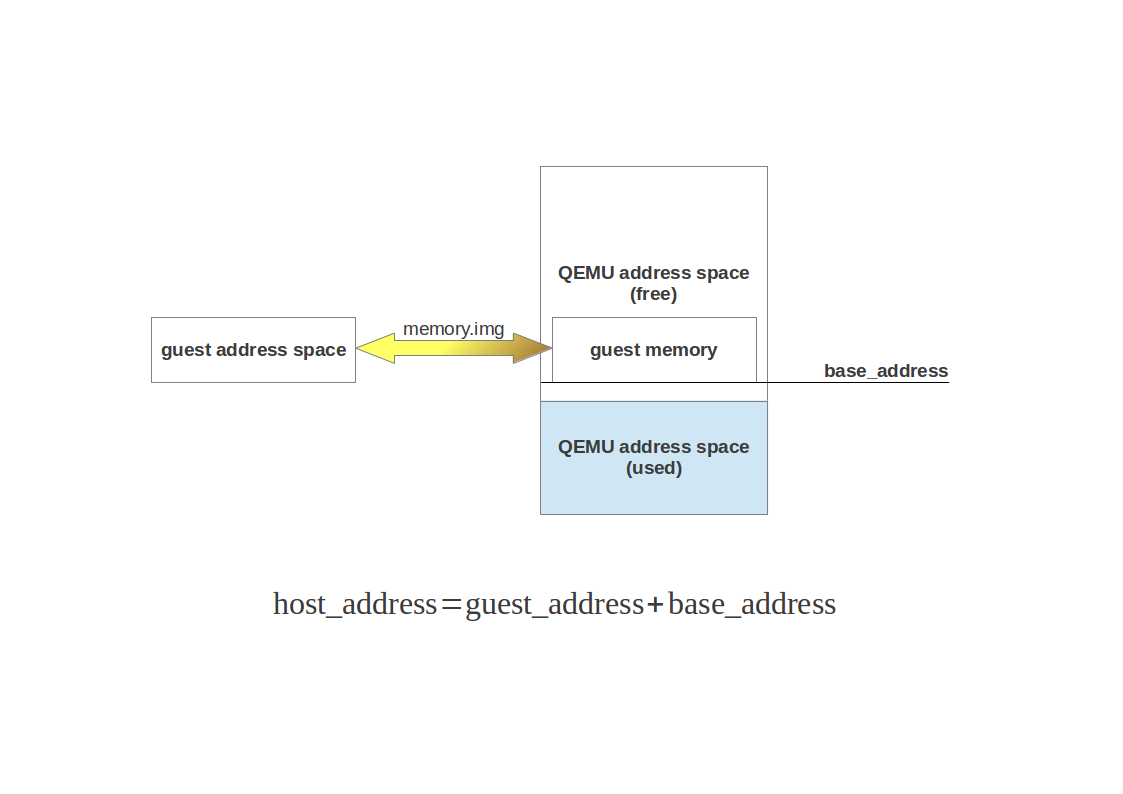
\includegraphics[width=1\linewidth]{qemu_memory_translation}}
\caption{Отображение памяти гостевого процесса в пространство адресов QEMU}
\label{pic:qemu_memory_translation}
\end{figure}

В режиме User Mode QEMU использует модель отображения адресного пространства гостя в адресное пространство хоста изображенную на рис.~\ref{pic:qemu_memory_translation}. Такая схема трансляции обеспечивает большую производительность, но при этом является плохо расширяемой. Например, при такой схеме трансляции недопустимо изменение расположения регионов памяти процесса друг относительно друга, а это создает проблему нехватки адресного пространства.

\paragraph{Проблема нехватки адресного пространства и ее решения.}\label{nomem}

Например, некоторый процесс, который необходимо мигрировать занимает суммарно в памяти 10 Mb. Эти 10 Mb разделяются между секциями бинарного файла программы, динамическими библиотеками, кучей и стеком процесса. Согласно рис.~\ref{pic:memory_layout}, стек процесса находится в самых верхних адресах пространства процесса, в то время как секции бинарного файла в нижних, поэтому при восстановлении процесса в памяти QEMU приходится запрашивать регион памяти размером \textit{stack\_start - code\_start} (см. листинг~\ref{code:mm_struct}). Естественно, такого региона в памяти процесса QEMU нет, так как QEMU использует свое адресное пространство также не локально.

Возможно несколько подходов к решению проблемы "нехватки" памяти. Рассмотрим два из них:

\begin{itemize}

    \item Реализация собственной модели трансляции памяти. Возможна реализация такой модели памяти, при которой отдельные участки адресного пространства QEMU видны гостевому процессу как непрерывный блок памяти. В частности, такую модель отображения реализуют ОС с поддержкой виртуальной памяти (при отображении виртуального адресного пространства процессов на физическую память), кроме того в режиме системной эмуляции QEMU также поддерживает такое отображение.

    Очевидными плюсами такого решения являются: рациональное использование памяти и высокая гибкость (например, часть памяти может быть сохранена в файл, т. е. может быть реализован \textit{swap} (или \textit{paging})~\footnote{http://en.wikipedia.org/wiki/Paging}).

    Очевидным недостатком такого решения является потеря производительности при трансляции адресов. Кроме того стоит отметить, что так как модель трансляции адресов интегрирована глубоко в кодогенертор QEMU, реализация этого решения требует внесения серьезных изменений в QEMU.

    \item Введение ограничений на мигрируемый процесс. Если заставить процесс использовать память последовательно (более компактно), то это решит проблему нехватки памяти. Добиться этого можно несколькими способами:

    \begin{itemize}

\begin{lstlisting}[caption=Резервирования места под стек в GCC Asm, label=code:reserve_stack]
    .data
        stack_end:
            .space  8192
        .set  stack_begin, .

    ...

    .text
        .globl  main
        .type  main,  @function

        main:

            # use custom stack segment
            leal   stack_begin, %esp
            movl   %esp,        %ebp

    ...
\end{lstlisting}



        \item сборка специального бинарного файла. Скомпоновав бинарный файл с библиотеками статически можно гарантировать, что в памяти процесса они будут расположены в нижней части адресного пространства.

        Для того, чтобы перенести стек процесса в нижнюю часть адресного пространства, можно зарезервировать память под стек в бинарном файле программы при компиляции, например, как это показано в листинге~\ref{code:reserve_stack}.

        Надо отметить, что резервирование стека не обязательно предусматривать в самом бинарном файле, для этого возможно разработать отдельное приложение, цель которого зарезервировать стек, после чего загрузить в память целевую программу (с помощью одного из вызовов exec).

        \item внесение изменений в ядро. Использование памяти процессом определяет ядро Linux (см. раздел~\ref{linux_memory}), поэтому возможно внести изменение в ядро, чтобы память процесса использовалась более локально.

        Эти изменения могут быть произведены как на стороне мигрируемого приложения, так и на стороне целевой платформы.

    \end{itemize}

\end{itemize}

В данной работе используется самый простой подход, при котором для тестов используется статически скомпонованный бинарный файл с явным резервированием сегмента стека. Такой подход позволяет быстро получить реализацию достаточную для проведения тестов производительности, кроме того он не требует вмешательств в ядро, что соответствует основным критериям, заявленным в разделе~\ref{aims}.

\paragraph{Резервирование и восстановление памяти гостевого процесса.}

Для резервирования памяти под гостевой процесс в QEMU User Mode существует функция \textit{init\_guest\_space}, определенная в файле \textit{linux-user/elfload.c}, в качестве аргументов функции передаются желаемый адрес начала блока (в данной работе он не используется), размер блока, смещение специальной памяти, выделенной для гостевых процессов (в данной работе не используется) и флаг, указывающий на то как интерпретировать желаемый адрес начала блока - как жесткое требование или рекомендацию (в данной работе также не используется).

Описание всех регионов памяти (см. рис.~\ref{pic:common_arch}) находится в файле \textit{memory.img} образа процесса. Формат файла определяется файлом описания protobuf. Таким образом загрузка памяти мигрируемого процесса в память QEMU состоит из следующих простых шагов:

\begin{enumerate}

    \item Чтение и разбор файла \textit{memory.img}
    \item Вычисление размера необходимого адресного пространства. Размер необходимого адресного пространства вычисляется как разница между самым высоким и самым низким адресами среди всех участков памяти, за исключением анонимных регионов и региона \textit{[vdso]}. Исключение этих регионов памяти безопасно для тестового приложения, однако для полнофункционального решения такой подход неприемлем.
    \item Резервирование адресного пространства с помощью вызова \textit{init\_guest\_space}.
    \item Копирование содержимого памяти гостевого процесса из файлов.

\end{enumerate}

\subsection{Восстановление регистров процессора}

Каждому frontend-у (см. раздел~\ref{qemu_dynamic_translator}) в QEMU соответствует структура описывающая соответствующий процессор, например, для \textit{x86} эта структура называется \textit{CPUX86State} и определена она в файле \textit{target-i386}. Эта структура содержит множество полей управляющих трансляцией, и именно она хранит контекст процесса.

\begin{lstlisting}[caption=Структура описывающая контекст, label=code:cpux86state]
    typedef struct CPUX86State {
        /* standard registers */
        target_ulong regs[CPU_NB_REGS];
        target_ulong eip;
        target_ulong eflags; /* eflags register. During CPU emulation, CC
                            flags and DF are set to zero because they are
                            stored elsewhere */

        ....        

    };
\end{lstlisting}


\begin{lstlisting}[caption=Индексы регистров x86\_32, label=code:regs_indexes]
#define R_EAX 0
#define R_ECX 1
#define R_EDX 2
#define R_EBX 3
#define R_ESP 4
#define R_EBP 5
#define R_ESI 6
#define R_EDI 7
\end{lstlisting}

В данной работе из всей структуры интересны лишь некоторые поля (см. листинг~\ref{code:cpux86state}). Каждому регистру общего назначения в массиве \textit{regs} соответствует свой индекс (см. листинг~\ref{code:regs_indexes}). Аналогичные массивы выделены под сегментные регистры, FPU стек, регистры mmx и xmm/sse.

Восстановление регистров процессора происходит по именам (см. интерфейс класса \textit{Register} на рис.~\ref{pic:suspend_arch}). Значение читаются из файла \textit{registers.img}. Формат файла определяется файлом описания protobuf (см. листинг~\ref{code:regs_proto}).


\section{Тестовый фреймворк}

\subsection{Системный вызовы Linux}\label{syscalls}

Интерфейс системных вызовов ОС Linux построен на программных прерываниях. Однако, с развитием аппаратных возможностей, появились альтернативные способы организации взаимодействия с ядром операционной системы, например, инструкции \textit{sysenter} и \textit{sysexit}, ускоряющие выполнение системных вызовов.

Для утилизации новых возможностей с целью ускорения системных вызовов была разработана виртуальная библиотека \textit{linux-vdso.so} (или \textit{linux-gate.so}). Такая библиотека является виртуальным динамическим разделяемым объектом (\textit{VDSO}), который распологается в адресном пространстве отдельного процесса. Задача этой библиотеки обеспечивать быстрые системные вызовы для конкретной платформы, например, \textit{libc} использует ее для выполнения системных вызовов. Но так как этой библиотеке не соответствует никакой файл разделяемой библиотеки, то статическая компоновка на нее не влияет, и регион \textit{VDSO} располагается в верхних регионах адресного пространства и не может быть восстановлен (см. раздел~\ref{nomem}).

В связи с этим при реализации тестового фреймворка нельзя пользоваться возможностями библиотеки \textit{libc} и все необходимые части необходимо реализовать самостоятельно.

\paragraph{Реализация обращения к системным вызовам.}

Системные вызовы на платформе Linux \textit{i386} используют прерывание с номером \textit{0x80}, номер системного вызова передается в регистре \textit{eax}, регистры \textit{ebx}, \textit{ecx} и \textit{edx} используются для передачи первых трех параметров системного вызова (для данной работы этого достаточно).

Для работы потребуются следующие системные вызовы:

\begin{itemize}

    \item \textit{write} - вывод в поток, с заданным файловым дескриптором

    \item \textit{getpid} - получение идентификатора процесса

    \item \textit{gettimeofday} - получение текущего системного времени, потенциально, с точностью до микросекунд.

\end{itemize}

\subparagraph{Системный вызов write.}

Системный вызов \textit{write} принимает три аргумента:

\begin{enumerate}
    \item файловый дескриптор
    \item указатель на блок данных для передачи
    \item размер блока данных в байтах
\end{enumerate}

\begin{lstlisting}[caption=Сигнатура функции write, label=code:sys_write]
long write_impl(unsigned long fd, const char * buf, unsigned long size);
\end{lstlisting}

Если во время выполнения системного вызова произошла ошибка, то возвращаемое значение будет меньше нуля и будет идентифицировать код ошибки, если же системный вызов выполнен удачно, будет возвращено количество записанных байт.

Системный вызов в тестовом фреймворке будет производится функцией с сигнатурой показанной в листинге~\ref{code:sys_write}

\subparagraph{Системный вызов getpid.} Системный вызов \textit{getpid} не принимает аргументов и возвращает одно число - идентификатор процесса. Номер системного вызова в Linux \textit{i386} - \textit{0x14}.

\begin{lstlisting}[caption=Сигнатура функции getpid, label=code:sys_getpid]
typedef int pid_t
pid_t getpid_impl();
\end{lstlisting}

Функция реализующая системный вызов в тестовом фреймворке имеет сигнатуру показанную в листинге~\ref{code:sys_getpid}.

\subparagraph{Системный вызов gettimeofday.}

Системный вызов \textit{gettimeofday} принимает два указателя на структуры \textit{timeval} и \textit{timezone} (см. листинг~\ref{code:sys_gettimeofday}) и заполняет структуры соответствующими данными.

\begin{lstlisting}[caption=Сигнатура функции gettimeofday, label=code:sys_gettimeofday]
typedef long time_t;
typedef long suseconds_t;

struct timeval
{
    time_t      tv_sec;
    suseconds_t tv_usec;
};

struct timezone
{
    int tz_minuteswest;
    int tz_dsttime;
};

long gettimeofday_impl(struct timeval * tv, struct timezone * tz);
\end{lstlisting}

Системному вызову соответствует номер \textit{0x4e} ОС Linux, в тестовом фреймворке ему соответствует функция с сигнатурой показанной в листинге~\ref{code:sys_gettimeofday}.
